\documentclass[11pt, a4paper]{article}

% Unicode + pełna obsługa polskich znaków (w tym pogrubienia i kursywy)
\usepackage{fontspec}
\usepackage{polyglossia}
\setdefaultlanguage{polish}
\setmainfont{lmroman10-regular.otf}[
    BoldFont=lmroman10-bold.otf,
    ItalicFont=lmroman10-italic.otf,
    BoldItalicFont=lmroman10-bolditalic.otf,
]
\defaultfontfeatures{Ligatures=TeX}

\usepackage{geometry}
\usepackage{graphicx}
\usepackage{titlesec}
\usepackage{hyperref}
\usepackage{booktabs}
\usepackage{array}
\usepackage{float}
\usepackage{caption}
\usepackage{longtable}
\usepackage{xcolor}
\usepackage{amsmath}
\usepackage{amssymb}
\usepackage[normalem]{ulem}

% Ścieżki do zasobów współdzielonych z konspektem
\graphicspath{{figures/}{../conspect/titlepage/}{titlepage/}}

% Page Geometry
\geometry{
    top=2.5cm,
    bottom=2.5cm,
    left=2.5cm,
    right=2.5cm
}

% Hyperlink Setup
\hypersetup{
    colorlinks=true,
    linkcolor=black,
    filecolor=magenta,
    urlcolor=blue,
    pdftitle={Raport końcowy - MCTS w zmodyfikowanym Connect4},
    pdfpagemode=FullScreen,
}

% Pomocnicze makra szablonu (usuń po uzupełnieniu treści)
\newcommand{\todo}[1]{\textcolor{red}{\textbf{[TODO: #1]}}}
\newcommand{\placeholder}[1]{\textit{[#1]}}

\begin{document}

%----------------------------------------------------------------------------------------
%	STRONA TYTUŁOWA
%----------------------------------------------------------------------------------------
\begin{titlepage}
    \centering

    
\includegraphics[width=0.9\textwidth]{logo_MINI_big(1).png}
    \vfill

    {\Large \bfseries Metody Sztucznej Inteligencji 2 \par}
    \vspace{0.8cm}
    {\LARGE \bfseries Raport końcowy \par}
    \vspace{0.8cm}
    {\Large \itshape Wykorzystanie i usprawnienie MCTS do implementacji sztucznej inteligencji grającej w \textit{Connect4} \par}

    \vfill

    \Large
    \textbf{Filip Filipkowski} \\
    \textbf{Antoni Kingston}

    \vfill
\end{titlepage}

%----------------------------------------------------------------------------------------
%	STRESZCZENIE
%----------------------------------------------------------------------------------------
\section*{Streszczenie}
\addcontentsline{toc}{section}{Streszczenie}

Raport przedstawia implementację i empiryczną ocenę agentów grających w zmodyfikowany wariant \textit{Connect4} typu \textit{suicide} na planszy $6 \times 8$ z ruchami \texttt{drop} i \texttt{push}. Zaimplementowano silnik gry, graczy opartych o minimax, Monte Carlo Tree Search w wariantach UCT, FPU, LGR i PMBp (tryb online, $1000$ iteracji na ruch), gracza losowego oraz interfejs do modeli językowych. Przeprowadzono turniej round-robin dziewięciu agentów (360 partii), wstępną ocenę jakości ruchów metryką \textit{Blunder Rate} względem przybliżonej wyroczni UCT oraz 70 partii człowiek--komputer z pięcioma uczestnikami.

W turnieju najwyższy \textit{Win Rate} osiągnął PMBp (76\%), przed UCT (65\%) i minimaxem $d{=}4$ (60\%); modele językowe zajęły ostatnie miejsca (6--11\%). PMBp wygrał bezpośrednie pojedynki z pozostałymi wariantami MCTS, co potwierdza hipotezę o skuteczności co najmniej jednej modyfikacji UCT; FPU i LGR nie poprawiły wyniku względem UCT. \textit{Blunder Rate} odróżnił słabych graczy od MCTS, lecz przy obecnej wyroczni (UCT, $20\,000$ iteracji) nie dostarczył danych wystarczających do rozstrzygnięcia hipotezy o odporności PMBp na pułapki taktyczne. W testach z człowiekiem (70 partii, pięciu uczestników) ludzie wygrali 28 partii, przegrali 31 i zremisowali 11; przeciwko wariantom MCTS --- 7 zwycięstw, 26 porażek i 7 remisów na 40 gier. Uczestnicy wygrali wszystkie partie z graczem losowym oraz osiem z dziesięciu z minimaxem $d{=}3$. Przewaga pierwszego gracza nie została wyeliminowana w sensie przyjętym w hipotezie (45--55\% \textit{Win Rate} jako czerwony). Ograniczenia obejmują liczbę partii na parę, przybliżony charakter wyroczni, brak treningu self-play przed turniejem oraz wąski zakres testów ludzkich i LLM.

\vspace{0.5cm}
\noindent\textbf{Słowa kluczowe:}
Monte Carlo Tree Search, UCT, Connect4, wariant suicide, First Play Urgency, Last Good Reply, Power-Mean Backpropagation, Blunder Rate

%----------------------------------------------------------------------------------------
%	SPIS TREŚCI
%----------------------------------------------------------------------------------------
\tableofcontents
\newpage

%----------------------------------------------------------------------------------------
%	1. OPIS PROBLEMU
%----------------------------------------------------------------------------------------
\section{Opis problemu}

Celem projektu jest empiryczne porównanie metod sztucznej inteligencji w grze złożonej taktycznie: zmodyfikowanym wariancie \textit{Connect4} typu \textit{suicide}. Badamy, czy i w jakim stopniu Monte Carlo Tree Search w wariancie UCT oraz jego modyfikacje (FPU, LGR, PMBp) przewyższają prostsze podejścia oraz---w szerszym ujęciu---jak wypadają względem człowieka i modeli językowych.

\subsection{Cel projektu}

Klasyczna gra \textit{Connect4} na planszy $6 \times 7$ została rozwiązana: pierwszy gracz może wymusić zwycięstwo przy optymalnej grze \cite{allis1988connectfour}. Dlatego w projekcie przyjmujemy bardziej złożony wariant \textit{suicide}, w którym celem jest uniknięcie utworzenia własnej linii czterech żetonów, a plansza ma wymiary $6 \times 8$. Dodatkowy ruch typu \texttt{push} oraz nietypowe kryterium końca partii zwiększają przestrzeń stanów i utrudniają stosowanie prostych heurystyk znanych z klasycznej wersji gry \cite{sheoran2022connect4}. Głównym pytaniem badawczym jest ocena skuteczności wariantów MCTS w takim środowisku oraz identyfikacja modyfikacji algorytmu, które realnie poprawiają jakość gry.

\subsection{Monte Carlo Tree Search i warianty UCT}
\label{sec:mcts-opis}

Monte Carlo Tree Search to metoda przeszukiwania drzewa decyzyjnego oparta na losowych symulacjach (rolloutach). W przeciwieństwie do minimaxa z ręcznie zaprojektowaną funkcją oceny, MCTS uczy się wartości pozycji na podstawie wyników wielu rozegranych partii próbnych \cite{browne2012survey}. Pojedyncza iteracja składa się z czterech faz: \textbf{wyboru} ścieżki od korzenia do liścia, \textbf{ekspansji} drzewa o nowy węzeł, \textbf{symulacji} losowej gry do stanu końcowego oraz \textbf{propagacji wstecznej} wyniku do odwiedzonych węzłów.

\subsubsection{UCT}

Podstawowym wariantem stosowanym w projekcie jest UCT (\textit{Upper Confidence Bound applied to Trees}) \cite{kocsis2006bandit}. W fazie wyboru preferowany jest ruch $a$ maksymalizujący:
\begin{equation*}
    \mathrm{UCT}(s, a) = \bar{X}_{s,a} + C \sqrt{\frac{\ln N(s)}{N(s,a)}},
\end{equation*}
gdzie $\bar{X}_{s,a}$ to średni wynik symulacji po ruchu $a$ ze stanu $s$, $N(s)$ i $N(s,a)$ oznaczają liczbę odwiedzin stanu i liczbę wykonań ruchu, a $C$ reguluje równowagę między eksploatacją (pierwszy składnik) a eksploracją (drugi składnik).

\subsubsection{FPU}

Modyfikacja \textit{First Play Urgency} dotyczy traktowania jeszcze nieodwiedzonych ruchów w fazie wyboru. Zamiast pomijać je do momentu pierwszej ekspansji, otrzymują one zadaną wartość początkową (parametr FPU), co pozwala kontrolować, jak agresywnie algorytm eksploruje nowe gałęzie drzewa \cite{cazenave2021batch}. Zbyt wysoka wartość FPU sprzyja płytkiemu przeszukiwaniu, zbyt niska --- przedwczesnej koncentracji na początkowo obiecujących liniach.

\subsubsection{LGR}

\textit{Last Good Reply} zmienia fazę symulacji: algorytm zapamiętuje ruchy, które w danej pozycji prowadziły do korzystnego wyniku, i preferuje je podczas kolejnych rolloutów \cite{drake2009lgr}. Celem jest ograniczenie szumu wynikającego z w pełni losowych symulacji bez wprowadzania pełnej heurystyki pozycyjnej.

\subsubsection{PMBp}

W standardowym MCTS wartość węzła to średnia arytmetyczna wyników symulacji. W wariancie \textit{Power-Mean Backpropagation} stosuje się średnią potęgową \cite{dam2020poweruct}:
\begin{equation*}
    V_p = \left(\frac{1}{k}\sum_{i=1}^k a_i^p\right)^{\frac{1}{p}},
\end{equation*}
gdzie $a_i$ to wyniki pojedynczych symulacji, a parametr $p$ steruje wpływem wartości skrajnych. Dla $p = 1$ otrzymujemy UCT w klasycznym wariancie backpropagation; im większe $p$, tym silniej ważymy zwycięstwa, im niższe tym silniej porażki.

\subsection{Badana modyfikacja gry Connect4}

\subsubsection{Wersja standardowa}

\textit{Connect4} to gra dwuosobowa, deterministyczna i z pełną informacją. W klasycznym wariancie na planszy $6 \times 7$ gracze na przemian wrzucają żetony do kolumn; żetony opadają na najniższe wolne pole. Wygrywa ten, kto pierwszy ułoży cztery własne żetony w jednej linii (poziomej, pionowej lub ukośnej). Plansze o innych proporcjach, np.\ $8 \times 6$, pojawiają się także w literaturze dotyczącej ogólnego programowania gier \cite{schiffel2010evaluation}.

\subsubsection{Wariant badany w projekcie}

W projekcie przyjmujemy wariant \textit{Don't Connect 4} (suicide). Poniżej zestawiono jego reguły.

\paragraph{Plansza i ruchy.}
Gra toczy się na planszy $6 \times 8$. W każdej turze gracz wykonuje jeden z dwóch typów ruchu w wybranej niepełnej kolumnie:
\begin{itemize}
    \item \texttt{drop} --- żeton spada na najniższe wolne pole kolumny (jak w klasycznym \textit{Connect4}),
    \item \texttt{push} --- żeton wpychany jest od spodu kolumny, a dotychczasowe żetony w tej kolumnie przesuwają się o jedno pole w górę.
\end{itemize}
Ruch \texttt{push} pozwala m.in.\ niszczyć istniejące układy na planszy, co znacząco zwiększa liczbę legalnych kontynuacji w porównaniu z samym \texttt{drop}.

\paragraph{Cel gry i liczenie linii.}
Gracz dąży do \emph{uniknięcia} utworzenia własnej linii czterech żetonów. 
\paragraph{Zakończenie partii.}
Obowiązuje reguła \textbf{natychmiastowej porażki właściciela linii}: jeśli w danym ruchu powstaje nowy segment czterech żetonów, przegrywa gracz, do którego należy ten segment---niezależnie od tego, kto wykonał ruch (własną linię lub wymuszenie przeciwnikowi). Jeżeli w jednym ruchu powstają linie obu graczy, partia kończy się \textbf{remisem}. Jeżeli w ruchu nie powstaje żadna nowa linia, gra trwa dalej aż do zapełnienia planszy, które skutkuje \textbf{remisem}.

\paragraph{Motywacja modyfikacji.}
Połączenie wariantu suicide, ruchu \texttt{push} i planszy $6 \times 8$ tworzy przestrzeń stanów trudniejszą do opanowania heurystyką typową dla klasycznego \textit{Connect4} (gdzie premiuje się własne zagrożenia ofensywne). Parzysta liczba kolumn łagodzi przewagę gracza rozpoczynającego wynikającą z zajęcia środka w wersji $6 \times 7$. Złożoność taktyczna wariantu---krótkoterminowe pułapki, wymuszanie linii przeciwnikowi, konieczność planowania skutków \texttt{push}---stanowi wymagające środowisko testowe dla algorytmów MCTS i ich modyfikacji.

%----------------------------------------------------------------------------------------
%	2. IMPLEMENTACJA APLIKACJI
%----------------------------------------------------------------------------------------
\section{Implementacja aplikacji}
\label{sec:implementacja}

Aplikacja została zaimplementowana w języku Python~3.11+ jako pakiet \texttt{connect4\_mcts} wraz ze skryptami pomocniczymi. Kod podzielono na warstwę logiki gry, moduł agentów, mechanizm rozgrywek oraz pipeline eksperymentalny. Projekt objęto testami automatycznymi weryfikującymi poprawność zasad gry, zachowanie agentów i spójność wyników turniejów.

\subsection{Architektura modułów}

Główne komponenty systemu przedstawia rysunek~\ref{fig:architektura}. Rdzeń stanowi silnik gry z niezmiennym modelem stanu (\texttt{GameState}), typem ruchu (\texttt{Move}) oraz logiką legalności i końca partii. Warstwa agentów implementuje wspólny protokół (\texttt{choose\_move}) dla gracza losowego, minimaxa, wariantów MCTS oraz modelu językowego. Moduł rozgrywek przeprowadza partie agent--agent, a interfejsy CLI i GUI udostępniają grę człowiekowi. Eksperymenty wsadowe obejmują turniej, ocenę \textit{Blunder Rate} oraz pełny pipeline eksperymentalny konfigurowany deklaratywnie (format TOML).

\begin{figure}[H]
    \centering
    \fbox{\parbox[c][5.5cm][c]{0.9\textwidth}{\centering
        Silnik gry $\rightarrow$ Agenci $\rightarrow$ Rozgrywki \\
        $\downarrow$ \quad\quad\quad $\downarrow$ \\
        CLI / GUI \quad Pipeline eksperymentalny
    }}
    \caption{Uproszczony przepływ zależności między modułami aplikacji.}
    \label{fig:architektura}
\end{figure}

\subsection{Silnik gry}

Stan gry reprezentowany jest jako niezmienny obiekt \texttt{GameState} zawierający planszę $6 \times 8$, gracza na ruchu oraz status partii. Metoda \texttt{apply\_move} została mocno zoptymalizowana, ze względu na stanowienie zdecydowanej większości obłożenia obliczeniowego: legalność ruchu sprawdzana jest w czasie $O(1)$, przebudowywane są wyłącznie zmienione komórki planszy, a nowe segmenty czterech żetonów wykrywane są inkrementalnie na podstawie różnicy stanów przed i po ruchu (zamiast pełnego skanowania planszy).

\subsection{Agenci i przeszukiwanie MCTS}

Wszyscy gracze implementują ten sam interfejs \texttt{Agent} z metodą \texttt{choose\_move(state)}. Fabryka agentów buduje graczy na podstawie nazwy typu (\texttt{random}, \texttt{minimax}, \texttt{uct}, \texttt{fpu}, \texttt{lgr}, \texttt{pmbp}, \texttt{llm}) oraz hiperparametrów przekazywanych z CLI, GUI lub konfiguracji eksperymentu.

\subsubsection{Gracze porównawczy}
\label{sec:gracze-porownawczy}

\textbf{Random} wybiera jednostajnie spośród legalnych ruchów \texttt{drop} i \texttt{push}.

\paragraph{Minimax z przycinaniem $\alpha$--$\beta$.}
Gracz \textbf{Minimax} przeszukuje drzewo ruchów do zadanej głębokości $d$ (parametr konfigurowalny; w turnieju \texttt{minimax-d3} ma $d=3$, \texttt{minimax-d4} ma $d=4$). W każdym węźle wybierany jest ruch maksymalizujący wartość heurystyczną z perspektywy gracza korzenia; na poziomach przeciwnika wartość jest minimalizowana. Stosowane jest przycinanie $\alpha$--$\beta$. Gdy $d=0$ lub brak legalnych kontynuacji, zwracana jest ocena liścia.

\paragraph{Funkcja oceny pozycji.}
Liście oraz pozycje nie rozstrzygnięte w ramach budżetu głębokości oceniane są dedykowaną funkcją oceny pozycji. Wynik podawany jest \emph{z perspektywy gracza, dla którego w danym momencie wykonywane jest przeszukiwanie} (gracza korzenia przy wyborze ruchu).

Dla stanu \textbf{terminalnego} (partia zakończona):
\begin{itemize}
    \item zwycięstwo ocenianego gracza: $+10^6$,
    \item porażka: $-10^6$,
    \item remis: $0$.
\end{itemize}
\noindent
Wartość terminalna zależy wyłącznie od zwycięzcy, a nie od liczby linii w wyniku końcowym.

Dla stanu \textbf{nieterminalnego}:
\begin{equation}
    H(s, p) = P(s, p_{\mathrm{opp}}) - P(s, p),
    \label{eq:minimax-heuristic}
\end{equation}
gdzie $p$ to oceniany gracz, $p_{\mathrm{opp}}$ --- jego przeciwnik, a $P(s, \cdot)$ --- \emph{potencjał linii} danego koloru w pozycji $s$. Jest to odwrócenie klasycznej heurystyki \textit{Connect4}: w wariancie suicide korzystna jest pozycja, w której \textbf{przeciwnik} ma duży potencjał zbudowania linii (można go do niej zmusić), a \textbf{własny} potencjał jest mały (unikamy tworzenia własnych zagrożeń).

\paragraph{Potencjał linii $P(s, c)$.}
Dla koloru $c$ funkcja sumuje wkłady wszystkich \emph{okien czterech pól} na planszy $6 \times 8$: każde okno to cztery sąsiednie komórki w jednym z czterech kierunków (poziomo, pionowo, po obu przekątnych). Dla okna $w$ niech $n_c$ i $n_{\mathrm{opp}}$ oznaczają liczbę żetonów odpowiednio koloru $c$ i przeciwnika w $w$. Jeśli $n_{\mathrm{opp}} > 0$, okno jest \textbf{pomijane} (linia tego koloru w tym miejscu jest zablokowana). W przeciwnym razie do sumy dodawana jest waga zależna od $n_c$:
\begin{center}
\begin{tabular}{cc}
    \toprule
    $n_c$ (żetony $c$ w oknie) & waga \\
    \midrule
    1 & 1 \\
    2 & 3 \\
    3 & 9 \\
    0 lub 4 & 0 \\
    \bottomrule
\end{tabular}
\end{center}
\noindent
Wagi rosną wykładniczo z liczbą własnych żetonów w otwartym oknie --- trzy żetony w jednym rzędzie bez blokady przeciwnika dają wkład $9$, co silnie karze zbliżanie się do własnej linii. Okna zawierające żeton przeciwnika nie wliczają się do potencjału danego koloru, co odzwierciedla niemożność dokończenia linii przez zablokowane układy.


\subsubsection{MCTS w trybie online}

Klasa \texttt{MCTSPlayer} realizuje cztery fazy MCTS opisane w sekcji~\ref{sec:mcts-opis}. W turniejach i GUI agenci działają w trybie \emph{online}: przed każdym ruchem wykonywany jest świeży cykl symulacji z zadanym budżetem iteracji, a drzewo nie jest utrzymywane między partiami (\texttt{begin\_new\_game} czyści stan przeszukiwania). Warianty FPU, LGR i PMBp różnią się odpowiednio fazą wyboru, polityką rolloutu oraz sposobem agregacji wyników w propagacji wstecznej.

Metoda \texttt{evaluate(state)} zwraca strukturę \texttt{SearchEvaluation} z wartością pozycji i oceną poszczególnych ruchów. Służy ona do liczenia metryki \textit{Blunder Rate}: przybliżona wyrocznia (silnik referencyjny z tagiem \texttt{ORACLE}) ocenia pozycje przed ruchem, a \textit{regret} mierzy spadek jakości względem ruchu wskazanego przez tę wyrocznię. Jakość tej metryki zależy wprost od siły i bezstronności wyroczni --- w projekcie jest to jedynie pierwsza, ograniczona próba jej zastosowania (szczegóły w sekcji~\ref{sec:wyrocznia}).

\subsubsection{Gracz LLM}

\texttt{LLMPlayer} komunikuje się z modelem językowym przez interfejs zgodny z API OpenAI (\texttt{OpenAIClient}). W każdej turze model reprezentację planszy oraz listę legalnych ruchów, a w pierwszej dodatkowo reguły gry; odpowiedź parsowana jest do obiektu \texttt{Move} i walidowana. Przy błędzie parsowania lub nielegalnym ruchu zapytanie jest ponawiane, a po wyczerpaniu prób stosowany jest fallback (losowy legalny ruch). Liczniki żądań i błędów zapisuje turniej do późniejszej analizy.

\subsection{Interfejsy użytkownika}

\textbf{CLI} umożliwia grę człowiek--agent lub demonstrację agent--agent z linii poleceń, z wyborem typu gracza i podstawowych hiperparametrów. \textbf{GUI} (Pygame) oferuje ekran ustawień (tryb jedno- lub dwuosobowy, wybór agenta, konfiguracja iteracji MCTS, głębokość minimaxa, parametry LLM) oraz interaktywną planszę z przełączaniem \texttt{drop}/\texttt{push}. Oba interfejsy korzystają z tego samego silnika gry i fabryki agentów.

\subsection{Pipeline eksperymentalny}

Eksperymenty turniejowe opisuje jeden plik konfiguracyjny w formacie TOML. Globalnie ustawia się m.in.\ ziarno generatora losowości, katalog wyjściowy i liczbę partii na parę; każdy uczestnik definiowany jest osobnym wpisem z typem oraz hiperparametrami (np.\ liczba iteracji MCTS, głębokość minimaxa, model LLM). Gracz oznaczony tagiem \texttt{ORACLE} służy wyłącznie do oceny blunderów i nie startuje w turnieju round-robin.

Pipeline rozgrywa każdą parę agentów określoną liczbę razy, naprzemiennie zamieniając kolory. Dla każdego ruchu zapisywany jest stan przed posunięciem, co umożliwia późniejszą ocenę wyrocznią. Wyniki agregowane są do tabel podsumowujących turniej. Osobny etap równolegle ocenia unikalne pozycje wyrocznią MCTS; pełny przebieg łączy turniej, analizę i---opcjonalnie---etap \textit{Blunder Rate} w jednym uruchomieniu z możliwością wznawiania.

%----------------------------------------------------------------------------------------
%	3. HIPOTEZY I EKSPERYMENTY
%----------------------------------------------------------------------------------------
\section{Sprawdzone hipotezy i opis eksperymentów}
\label{sec:hipotezy}

W niniejszej sekcji zestawiamy hipotezy sformułowane w konspekcie projektu (dostosowane do faktycznie zaimplementowanych reguł gry) oraz opisujemy przeprowadzone eksperymenty: automatyczny turniej agentów, ocenę \textit{Blunder Rate} wyrocznią MCTS oraz testy człowiek--komputer z udziałem pięciu graczy. Szczegóły implementacji agentów i pipeline'u znajdują się w sekcji~\ref{sec:implementacja}; wyniki liczbowe --- w sekcji~4.

\subsection{Postawione hipotezy}
\label{sec:hipotezy-sformulowanie}

\begin{enumerate}
    \item \textbf{Supremacja nad ludźmi i LLM.}
    Warianty MCTS z budżetem $1000$ iteracji na ruch (tryb online, bez trwałego drzewa między partiami) osiągają wyższą skuteczność niż lokalnie uruchomione modele językowe oraz niż amatorzy w testach człowiek--komputer, wygrywając z nimi w ponad $75\%$ rozgrywek w warunkach opisanych w sekcji~\ref{sec:metodyka}.

    \item \textbf{Przewaga UCT nad graczem heurystycznym.}
    Gracz MCTS w wariancie UCT z budżetem $1000$ iteracji na ruch osiąga wyższy \textit{Win Rate} w turnieju round-robin niż minimax z heurystyką dostosowaną do wariantu suicide (przynajmniej przy głębokości $d=4$, reprezentującej najmocniejszą wersję heurystyczną w naszym zestawie).

    \item \textbf{Odporność PMBp na pułapki taktyczne.}
    Modyfikacja \textit{Power-Mean Backpropagation} z parametrem $p = 2{,}5$ wykazuje istotnie niższą tendencję do rażących błędów (\textit{Blunder Rate}) niż pozostałe warianty MCTS przy tym samym budżecie iteracji --- przy założeniu wiarygodnej wyroczni oceniającej jakość pozycji (hipoteza weryfikowalna tylko w takim stopniu, w jakim spełniony jest ten warunek).

    \item \textbf{Zbalansowanie rozgrywki.}
    Plansza $6 \times 8$ w połączeniu z regułą natychmiastowej porażki właściciela nowej linii nie wprowadza dominującej przewagi pierwszego gracza: \textit{Win Rate} rozegranych jako czerwony (pierwszy ruch) mieści się w przybliżeniu w przedziale $45\%$--$55\%$ dla silnych agentów, a udział remisów pozostaje istotny zwłaszcza w parach MCTS--MCTS.

    \item \textbf{Skuteczność modyfikacji UCT.}
    Co najmniej jedna z badanych modyfikacji UCT (FPU, LGR lub PMBp) osiąga wyższy \textit{Win Rate} w turnieju końcowym niż bazowy UCT przy identycznym budżecie $1000$ iteracji na ruch.
\end{enumerate}

\noindent
Uwaga metodologiczna: w konspekcie rozważano mechanizm \emph{sprawiedliwości turowej}; w ostatecznej implementacji przyjęto regułę \textbf{natychmiastowej porażki właściciela linii} (sekcja~1). Hipoteza~4 weryfikowana jest zatem przez analizę \textit{Win Rate} w podziale na kolor startowy oraz \textit{Draw Rate}, a nie przez osobny mechanizm gry.

\subsection{Porównywani gracze}
\label{sec:gracze}

Eksperyment końcowy obejmował dziewięciu uczestników turnieju oraz jedną wyrocznię pomocniczą. Tabela~\ref{tab:players} zestawia ich typy i hiperparametry. Wszyscy gracze MCTS w turnieju działali w trybie \emph{online}: przed każdym ruchem wykonywano świeże przeszukiwanie z podanym budżetem iteracji, bez utrzymywania drzewa między partiami (por. sekcja~\ref{sec:implementacja}).

\begin{table}[H]
    \centering
    \caption{Skład turnieju końcowego --- identyfikatory z konfiguracji TOML.}
    \label{tab:players}
    \small
    \begin{tabular}{lll}
        \toprule
        \textbf{Identyfikator} & \textbf{Typ} & \textbf{Parametry} \\
        \midrule
        \texttt{uct-1000-1.41} & UCT & $1000$ iter./ruch, $C = 1{,}41$ \\
        \texttt{fpu-1000-1.0} & FPU & $1000$ iter./ruch, $\mathrm{FPU} = 1{,}0$ \\
        \texttt{pmbp-1000-2.5} & PMBp & $1000$ iter./ruch, $p = 2{,}5$ \\
        \texttt{lgr-1000} & LGR & $1000$ iter./ruch \\
        \texttt{minimax-d4} & Minimax & głębokość $d = 4$ \\
        \texttt{minimax-d3} & Minimax & głębokość $d = 3$ \\
        \texttt{random} & Losowy & --- \\
        \texttt{qwen2.5} & LLM & \texttt{qwen2.5:7b}, Ollama, $T{=}1$ \\
        \texttt{openchat} & LLM & \texttt{openchat:7b}, Ollama, $T{=}1$ \\
        \texttt{uct-20000-1.0-ORACLE} & Wyrocznia (UCT) & tag \texttt{ORACLE}, $20\,000$ iter./pozycja \\
        \bottomrule
    \end{tabular}
\end{table}

Gracz oznaczony tagiem \texttt{ORACLE} nie brał udziału w turnieju round-robin --- służył wyłącznie do oceny jakości ruchów (\textit{Blunder Rate}). Modele językowe komunikowały się z lokalnym serwerem Ollama (interfejs zgodny z API OpenAI); w turnieju automatycznym uruchamiano je bez dodatkowego \emph{chain-of-thought}, z walidacją i ponawianiem nielegalnych odpowiedzi (szczegóły w sekcji~\ref{sec:implementacja}).

\subsection{Metodyka eksperymentalna}
\label{sec:metodyka}

\subsubsection{Turniej automatyczny round-robin}

Główny eksperyment przeprowadzono z użyciem opisanej wyżej konfiguracji turniejowej. Dla każdej nieuporządkowanej pary graczy rozegrano \textbf{10 partii}, przy naprzemiennym przypisywaniu kolorów (pięć partii jako czerwony, pięć jako żółty). Łącznie wykonano $ \binom{9}{2} \times 10 = 360$ gier.

Ziarno generatora losowości ustawiono na $0$; dla partii $i$ w parze $(A, B)$ stosowano deterministyczne ziarno wyliczane z indeksu pary i numeru gry, co umożliwia odtworzenie przebiegu turnieju. Dla każdej partii zapisywano m.in.\ identyfikator pary, wynik, liczbę ruchów, czasy decyzji obu agentów oraz --- w przypadku LLM --- liczbę zapytań i błędów parsowania. Pełny stan przed każdym ruchem stanowi podstawę późniejszej oceny wyrocznią.

\subsubsection{Wyrocznia i metryka Blunder Rate}
\label{sec:wyrocznia}

W projekcie przyjęto \textbf{przybliżoną} wyrocznię do oceny jakości ruchów --- nie jest to silnik uznawany za optymalny w sensie teoretycznym, lecz pierwsza praktyczna próba zastosowania metryki \textit{Blunder Rate} w tym wariancie gry. Świadome ograniczenia tej próby należy brać pod uwagę przy interpretacji hipotezy~3 i wszystkich wyników dotyczących blunderów.

\paragraph{Konstrukcja wyroczni.}
Silnik referencyjny to zwykły UCT (bez FPU/LGR/PMBp). Przy ocenie pozycji z turnieju stosowano $20\,000$ iteracji na stan --- więcej niż agenci turniejowi ($1000$/ruch), lecz nadal skończony budżet Monte Carlo.

\paragraph{Definicja blundera.}
Ruch uznaje się za \textbf{blunder}, jeśli wartość pozycji po wybranym ruchu (w skali $[0,1]$) jest o więcej niż $\tau = 0{,}3$ niższa od wartości ruchu wskazanego przez wyrocznię. \textit{Blunder Rate} to odsetek takich ruchów; \textit{regret} to średnia różnica wartości między ruchem wyroczni a ruchem agenta.

\paragraph{Ułomności pomiaru.}
\begin{itemize}
    \item Wyrocznia sama jest UCT-em --- może \emph{systematycznie faworyzować} ocenę ruchów podobnych do własnej polityki i niedoszacowywać wartość strategii charakterystycznych dla PMBp, FPU lub LGR.
    \item $20\,000$ iteracji to kompromis między czasem obliczeń a stabilnością oceny; nie ma gwarancji zbieżności wartości korzenia do „prawdziwej” jakości pozycji w tak złożonym wariancie.
    \item Drzewo wyroczni budowane było w self-playu UCT-a i może \emph{słabo pokrywać} pozycje osiągane przez innych agentów w turnieju.
    \item Próg $\tau = 0{,}3$ jest arbitralny; przy silnych agentach MCTS odsetek blunderów spada do ok.\ 0{,}1--0{,}2\%, co daje \textbf{liczbę pojedynczych zdarzeń} (1--9 na tysiąc ruchów) --- zbyt mało, by wiarygodnie rozróżniać warianty MCTS bez znacznie większej próby i lepszej wyroczni.
\end{itemize}

\noindent
Z powyższych powodów wyniki \textit{Blunder Rate} traktujemy jako \textbf{material pomocniczy i eksploracyjny}, a nie jako rozstrzygające dowody na korzyść lub niekorzyść któregokolwiek wariantu MCTS w sensie hipotezy~3.

\subsubsection{Porównanie z modelami językowymi}

W turnieju automatycznym uczestniczyły dwa modele uruchomione lokalnie: \texttt{qwen2.5:7b} oraz \texttt{openchat:7b}. Każdy model rozegrał po 80 partii (po 10 z każdym z pozostałych ośmiu przeciwników). Zebrano metryki niezawodności interfejsu (odsetek niepoprawnych odpowiedzi, udział ruchów losowych po wyczerpaniu ponowień).

\subsection{Testy człowiek--komputer}
\label{sec:testy-czlowiek}

Uzupełnieniem turnieju automatycznego były \textbf{testy z udziałem pięciu graczy ludzkich}. Każda osoba rozgrywała partie przeciwko wybranym agentom za pośrednictwem graficznego interfejsu użytkownika (Pygame). Uczestnik wybierał kolor (\texttt{drop}/\texttt{push}, kolumna) zgodnie z tymi samymi regułami wariantu suicide co w turnieju maszynowym; przeciwnik był konfigurowany z poziomu GUI (typ agenta oraz hiperparametry, np.\ liczba iteracji MCTS lub głębokość minimaxa).

Protokół testów:
\begin{itemize}
    \item \textbf{Liczba uczestników:} 5 absolwentów kierunków technicznych z tytułem inżyniera bez wcześniejszego treningu w tym wariancie gry (poza krótkim wprowadzeniem do zasad). 
    \item \textbf{Przeciwnicy:} siedmiu agentów z turnieju końcowego --- \texttt{random}, minimax (\texttt{minimax-d3}, \texttt{minimax-d4}) oraz cztery warianty MCTS (\texttt{uct-1000-1.41}, \texttt{fpu-1000-1.0}, \texttt{pmbp-1000-2.5}, \texttt{lgr-1000}) z tymi samymi hiperparametrami co w turnieju automatycznym.
    \item \textbf{Organizacja partii:} każdy uczestnik rozgrywał \textbf{dwie} partie z każdym agentem --- raz jako czerwony, raz jako żółty --- łącznie $5 \times 7 \times 2 = 70$ gier.
    \item \textbf{Cel:} weryfikacja hipotezy~1 (supremacja MCTS nad człowiekiem) oraz jakościowe porównanie trudności gry dla człowieka z wynikami turnieju agentów.
\end{itemize}

\subsection{Metryki oceny}
\label{sec:metryki}

Do weryfikacji hipotez wykorzystano następujące metryki (zgodnie z metodologią z konspektu, w zakresie faktycznie zaimplementowanym w pipeline'ie):

\begin{itemize}
    \item \textbf{Win Rate} --- odsetek partii zakończonych zwycięstwem danego gracza; liczony łącznie oraz osobno dla gier jako czerwony i jako żółty (\textit{side balance}).

    \item \textbf{Draw Rate} --- odsetek remisów; istotny przy ocenie zbalansowania wariantu (hipoteza~4) oraz strategii defensywnych.

    \item \textbf{Średnia długość partii} --- liczba ruchów do zakończenia gry; krótkie partie często wskazują na szybkie wykorzystanie pułapki taktycznej lub rażący błąd.

    \item \textbf{Czas decyzji} --- średni czas wyboru ruchu [s]; porównanie kosztu obliczeniowego MCTS, minimaxa i LLM.

    \item \textbf{Blunder Rate} --- odsetek ruchów z $\mathrm{regret} > \tau = 0{,}3$ względem przybliżonej wyroczni UCT ($20\,000$ iteracji); metryka pomocnicza przy weryfikacji hipotezy~3, o ograniczonej mocy rozróżniającej (sekcja~\ref{sec:wyrocznia}).

    \item \textbf{Średni regret} --- średnia strata wartości pozycji względem ruchu wskazanego przez wyrocznię; podlega tym samym zastrzeżeniom co \textit{Blunder Rate}.

    \item \textbf{Metryki LLM} --- odsetek niepoprawnych odpowiedzi modelu i udział ruchów losowych po błędzie.
\end{itemize}

\noindent
Tabela~\ref{tab:hipotezy-metryki} wiąże hipotezy z eksperymentami i metrykami weryfikacji.

\begin{table}[H]
    \centering
    \caption{Mapowanie hipotez na eksperymenty i metryki.}
    \label{tab:hipotezy-metryki}
    \small
    \begin{tabular}{p{4.2cm}p{4.8cm}p{4.5cm}}
        \toprule
        \textbf{Hipoteza} & \textbf{Eksperyment} & \textbf{Metryki} \\
        \midrule
        1. Supremacja nad ludźmi i LLM &
        Turniej automatyczny + testy człowiek--komputer &
        Win Rate agenta $>$ $75\%$ \emph{vs} LLM i człowiek \\
        2. UCT \emph{vs} minimax &
        Pary UCT--minimax w turnieju &
        Win Rate, bezpośrednie pojedynki \\
        3. Odporność PMBp &
        Ocena \textit{Blunder Rate} (wyrocznia UCT) &
        Blunder Rate --- przy zastrzeżeniach sekcji~\ref{sec:wyrocznia} \\
        4. Zbalansowanie &
        Wszystkie pary turnieju + testy człowiek--komputer &
        Win Rate wg koloru, Draw Rate \\
        5. Modyfikacje UCT &
        Ranking turniejowy, pary MCTS &
        Win Rate PMBp/FPU/LGR \emph{vs} UCT \\
        \bottomrule
    \end{tabular}
\end{table}

%----------------------------------------------------------------------------------------
%	4. WYNIKI EKSPERYMENTÓW
%----------------------------------------------------------------------------------------
\section{Wyniki eksperymentów}

Poniżej przedstawiamy wyniki eksperymentu końcowego: turnieju round-robin dziewięciu agentów (360 partii), wstępnej oceny \textit{Blunder Rate} na ok.\ 9400 ruchach (z zastrzeżeniami co do wyroczni, sekcja~\ref{sec:wyrocznia}) oraz testów z pięcioma graczami ludzkimi i porównania z modelami językowymi.

\subsection{Wyniki turnieju agentów}

Turniej round-robin rozegrano w układzie dziewięciu graczy, po 80 partii na agenta. Ranking według \textit{Win Rate} przedstawia tabela~\ref{tab:tournament-summary} i rysunek~\ref{fig:standings-win-rate}. Pierwsze trzy miejsca zajęli PMBp (76{,}3\%, 61 wygranych na 80), UCT (65{,}0\%) oraz minimax $d{=}4$ (60{,}0\%); kolejne pozycje: LGR (57{,}5\%), FPU (56{,}3\%), minimax $d{=}3$ (46{,}3\%), gracz losowy (18{,}8\%), OpenChat (11{,}3\%), Qwen 2.5 (6{,}3\%).

\begin{figure}[H]
    \centering
    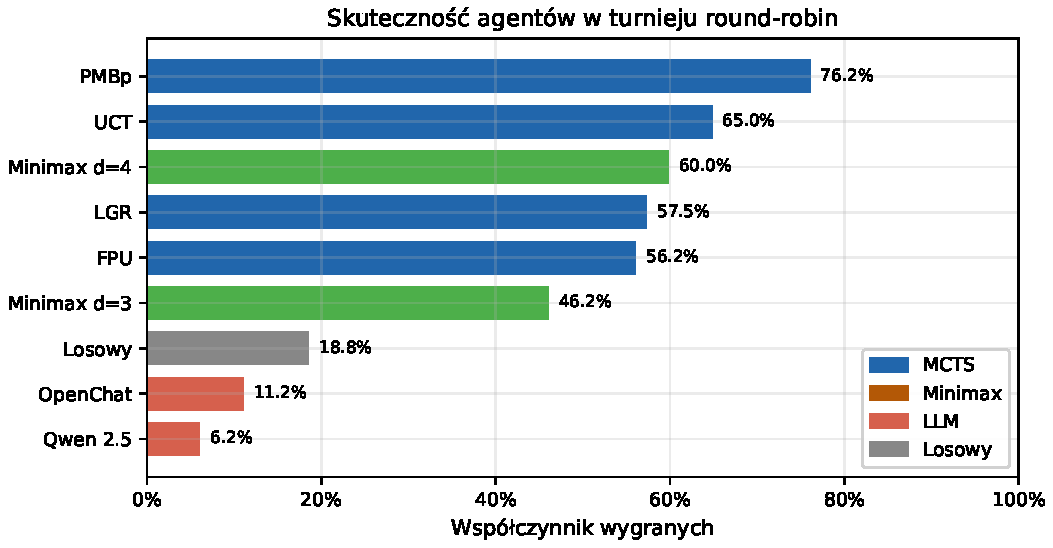
\includegraphics[width=0.88\textwidth]{figures/standings_win_rate.pdf}
    \caption{Skuteczność agentów w turnieju round-robin (80 partii na gracza).}
    \label{fig:standings-win-rate}
\end{figure}

\begin{figure}[H]
    \centering
    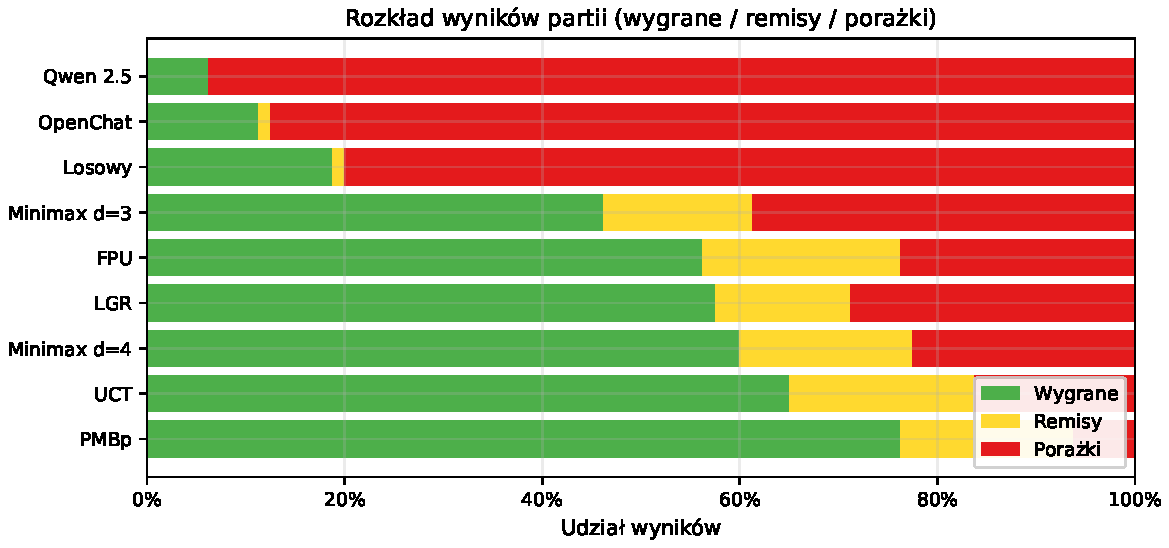
\includegraphics[width=0.92\textwidth]{figures/standings_outcomes.pdf}
    \caption{Rozkład wyników: wygrane, remisy i porażki według agenta.}
    \label{fig:standings-outcomes}
\end{figure}

\begin{table}[H]
    \centering
    \caption{Podsumowanie turnieju końcowego.}
    \label{tab:tournament-summary}
    \small
    \begin{tabular}{lrrrrr}
        \toprule
        \textbf{Gracz} & \textbf{M.} & \textbf{Win rate} & \textbf{Draw rate} & \textbf{Śr.\ ruchów} & \textbf{Śr.\ czas [s]} \\
        \midrule
        PMBp & 1 & 76{,}3\% & 17{,}5\% & 30{,}4 & 1{,}28 \\
        UCT & 2 & 65{,}0\% & 18{,}8\% & 30{,}2 & 1{,}26 \\
        Minimax $d{=}4$ & 3 & 60{,}0\% & 17{,}5\% & 31{,}7 & 0{,}63 \\
        LGR & 4 & 57{,}5\% & 13{,}8\% & 31{,}1 & 0{,}96 \\
        FPU & 5 & 56{,}3\% & 20{,}0\% & 29{,}9 & 1{,}51 \\
        Minimax $d{=}3$ & 6 & 46{,}3\% & 15{,}0\% & 31{,}6 & 0{,}13 \\
        Losowy & 7 & 18{,}8\% & 1{,}3\% & 18{,}4 & $\approx 0$ \\
        OpenChat & 8 & 11{,}3\% & 1{,}3\% & 18{,}2 & 0{,}65 \\
        Qwen 2.5 & 9 & 6{,}3\% & 0{,}0\% & 13{,}3 & 0{,}56 \\
        \bottomrule
    \end{tabular}
\end{table}

Średnia długość partii wynosiła ok.\ 30--32 ruchy u agentów MCTS i minimaxa oraz ok.\ 13--18 ruchów w grach z udziałem LLM lub gracza losowego. W turnieju PMBp zanotował 61 zwycięstw, 14 remisów i 5 porażek na 80 partii.

\paragraph{Zbalansowanie kolorów startowych.}
Rysunek~\ref{fig:side-balance} zestawia \textit{Win Rate} w podziale na kolor startowy (czerwony = pierwszy ruch). Dla PMBp wartości wynoszą 72{,}5\% (czerwony) i 80{,}0\% (żółty); dla UCT --- 67{,}5\% i 62{,}5\%. U części pozostałych agentów oba wskaźniki są bliższe siebie.

\begin{figure}[H]
    \centering
    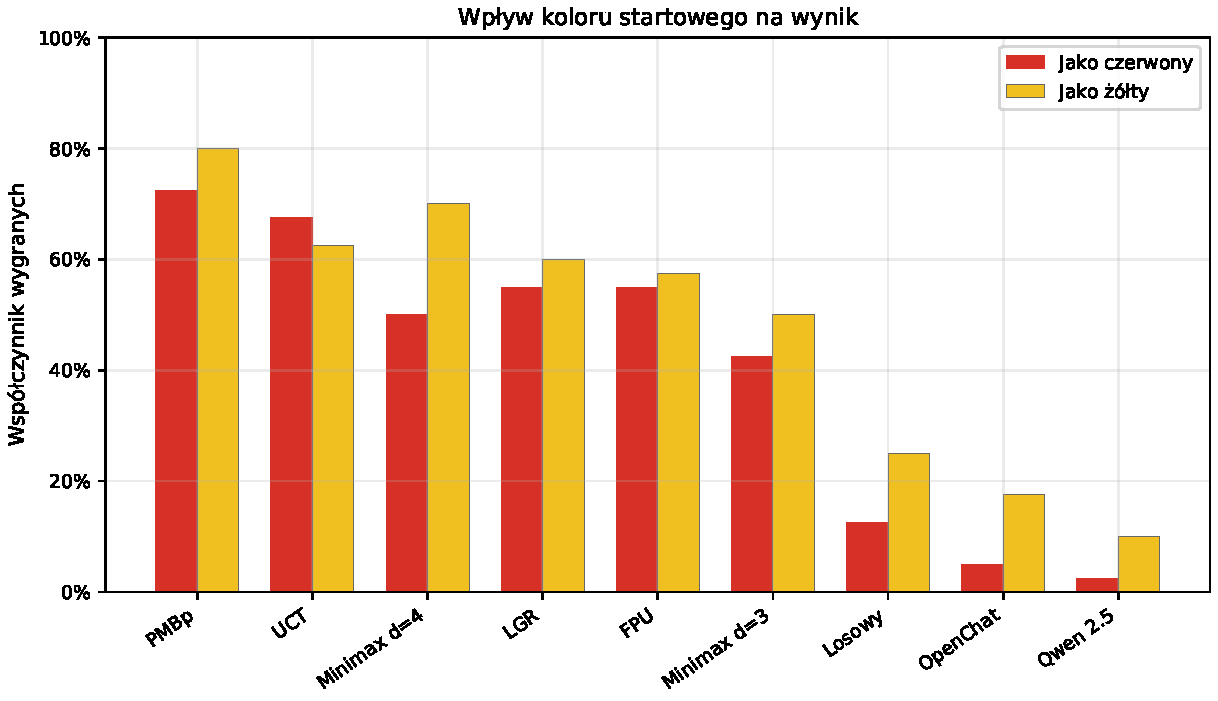
\includegraphics[width=0.92\textwidth]{figures/side_balance.pdf}
    \caption{Współczynnik wygranych w zależności od koloru startowego (czerwony = pierwszy ruch).}
    \label{fig:side-balance}
\end{figure}

\begin{figure}[H]
    \centering
    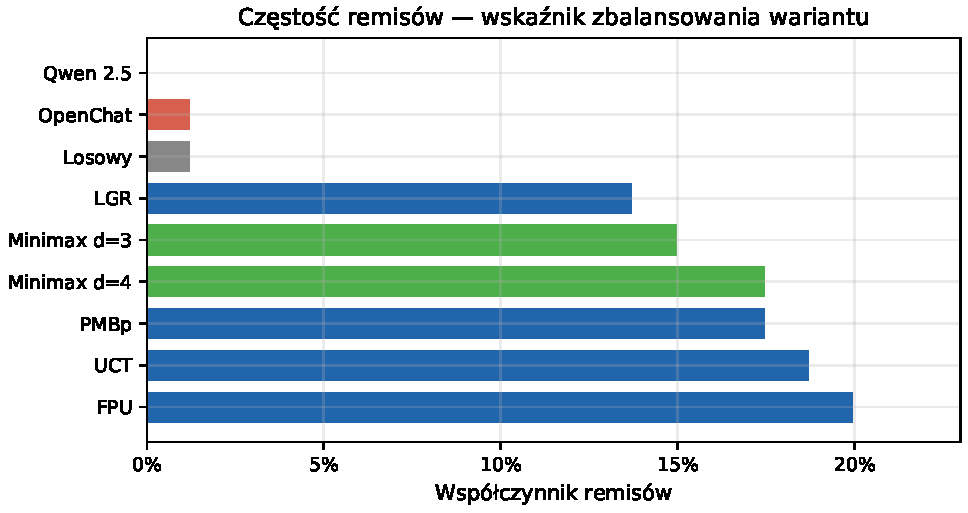
\includegraphics[width=0.85\textwidth]{figures/draw_rate.pdf}
    \caption{Częstość remisów według agenta.}
    \label{fig:draw-rate}
\end{figure}

\begin{figure}[H]
    \centering
    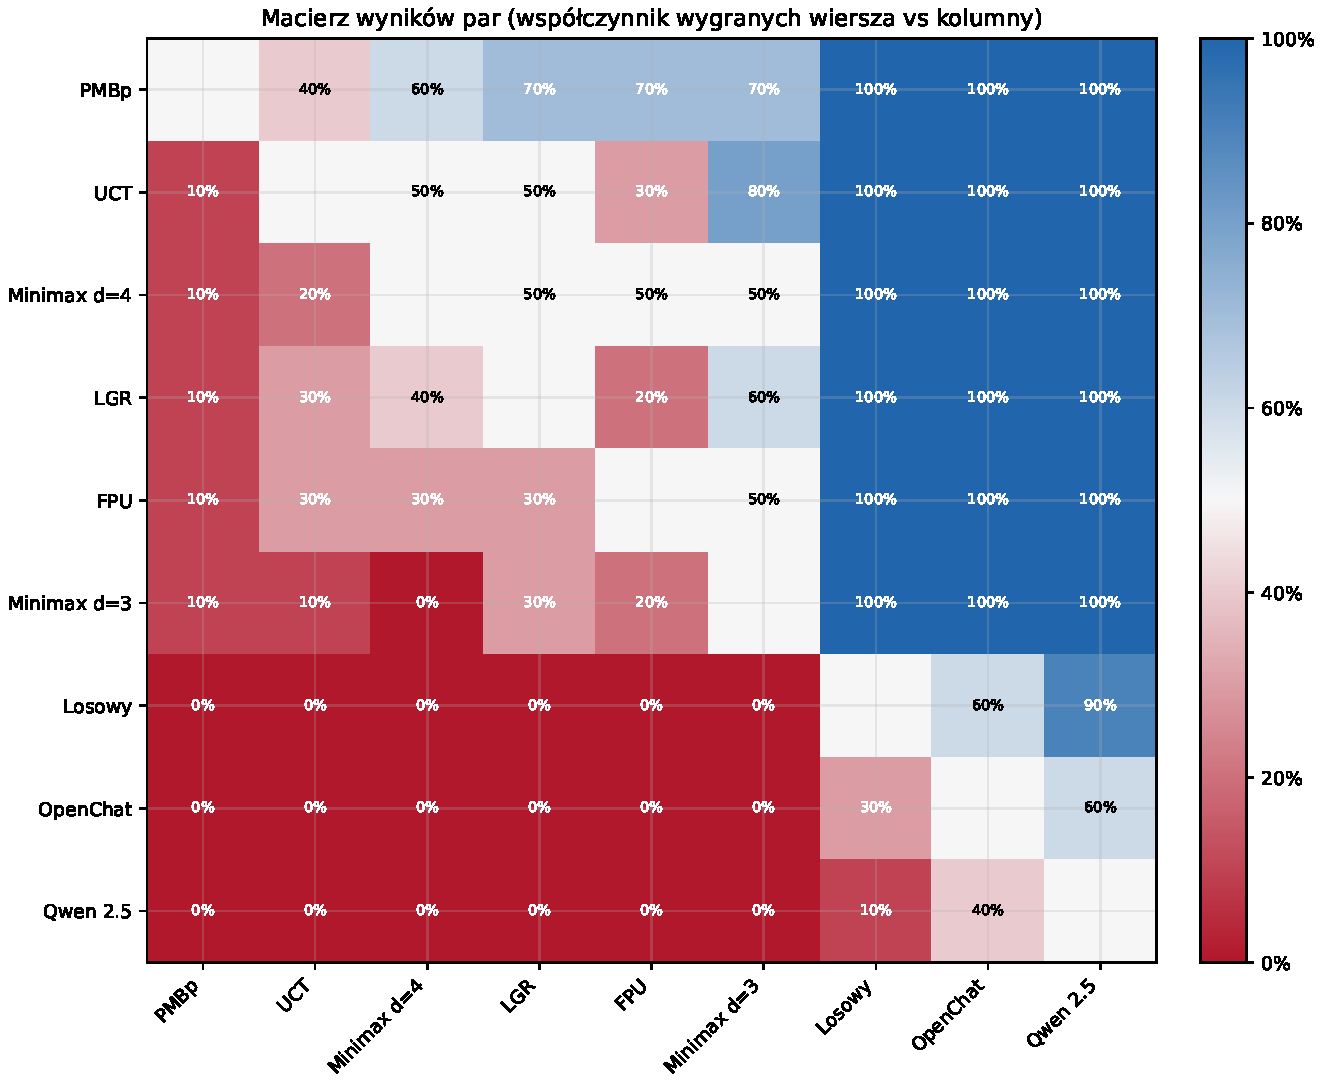
\includegraphics[width=0.95\textwidth]{figures/matchup_heatmap.pdf}
    \caption{Macierz wyników par: wartość w komórce $(i,j)$ to \textit{Win Rate} gracza wiersza przeciwko graczowi kolumny.}
    \label{fig:matchup-heatmap}
\end{figure}

\subsection{Porównanie wariantów MCTS}

Cztery warianty MCTS miały identyczny budżet $1000$ iteracji na ruch. Tabela~\ref{tab:mcts-head-to-head} zestawia bezpośrednie pojedynki; rysunek~\ref{fig:mcts-head-to-head} pokazuje je w formie macierzy.

\begin{table}[H]
    \centering
    \caption{Wybrane pary bezpośrednie między wariantami MCTS (format: wygrane--przegrane--remisy przy 10 grach).}
    \label{tab:mcts-head-to-head}
    \begin{tabular}{lcc}
        \toprule
        \textbf{Para} & \textbf{Wynik} & \textbf{Draw rate} \\
        \midrule
        PMBp \emph{vs} LGR & 7--1--2 & 20\% \\
        PMBp \emph{vs} FPU & 7--1--2 & 20\% \\
        PMBp \emph{vs} UCT & 4--1--5 & 50\% \\
        UCT \emph{vs} LGR & 5--3--2 & 20\% \\
        UCT \emph{vs} FPU & 3--3--4 & 40\% \\
        FPU \emph{vs} LGR & 3--2--5 & 50\% \\
        \bottomrule
    \end{tabular}
\end{table}

\begin{figure}[H]
    \centering
    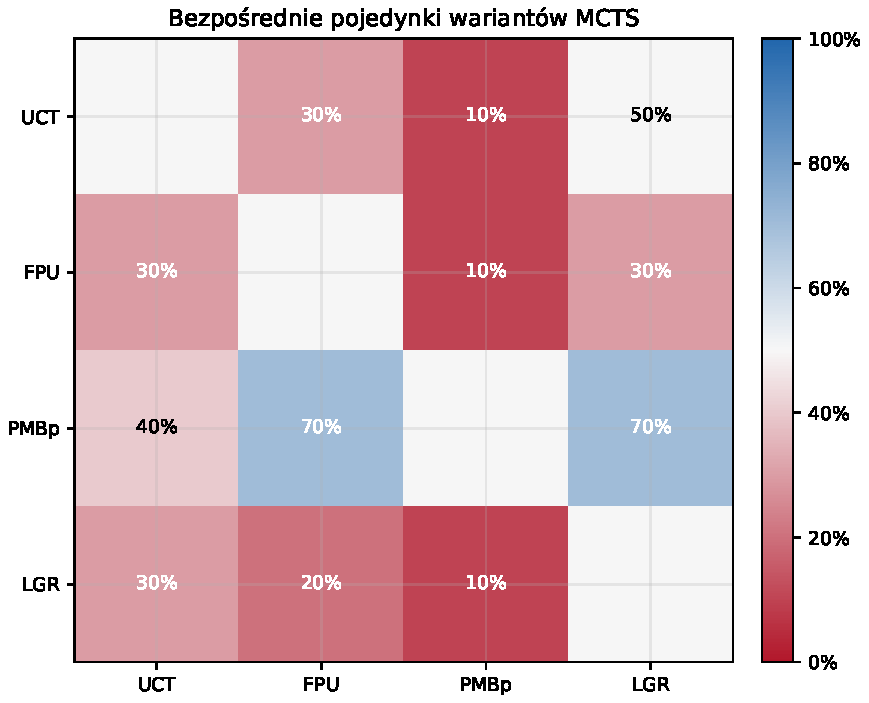
\includegraphics[width=0.72\textwidth]{figures/mcts_head_to_head.pdf}
    \caption{Bezpośrednie pojedynki UCT, FPU, PMBp i LGR.}
    \label{fig:mcts-head-to-head}
\end{figure}

W parach między wariantami MCTS (po 10 gier na parę) PMBp uzyskał łącznie 18 zwycięstw, 3 porażki i 9 remisów. W bezpośrednim pojedynku PMBp--UCT wynik wyniósł 4--1--5, PMBp--FPU 7--1--2, PMBp--LGR 7--1--2, UCT--LGR 5--3--2, UCT--FPU 3--3--4, FPU--LGR 3--2--5. W parach UCT--minimax $d{=}3$ i UCT--minimax $d{=}4$ odpowiednio 8--1--1 oraz 5--2--3; w parach PMBp--minimax $d{=}3$ i PMBp--minimax $d{=}4$ --- 7--1--2 oraz 6--1--3. Średni czas decyzji minimaxa wynosił 0{,}13--0{,}63\,s na ruch, MCTS ok.\ 1{,}3\,s.

\begin{figure}[H]
    \centering
    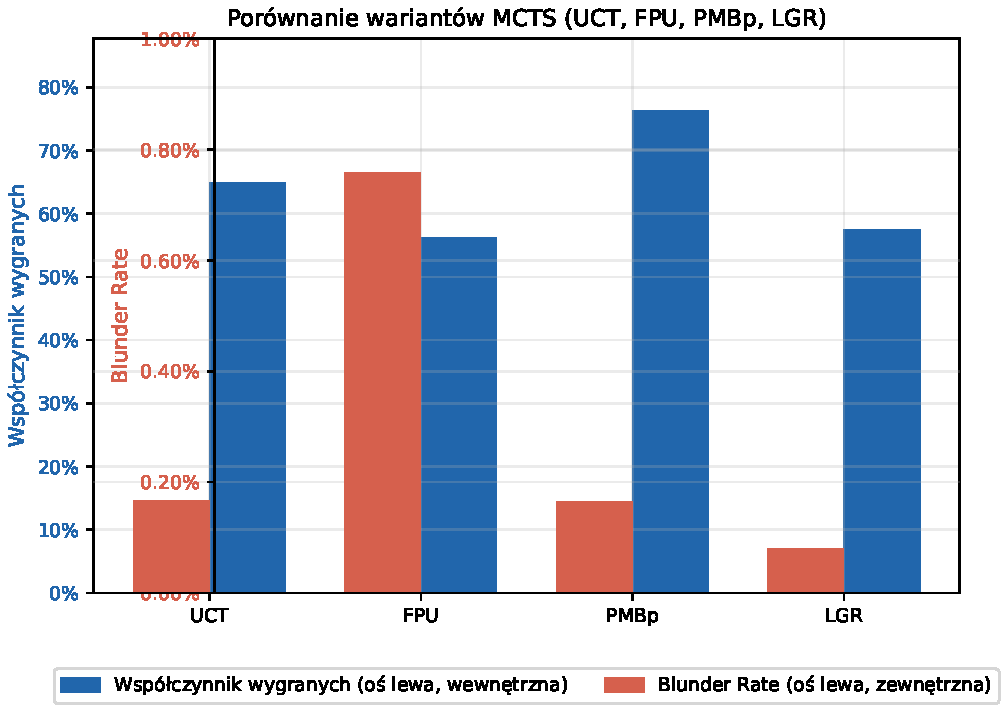
\includegraphics[width=0.88\textwidth]{figures/mcts_variants.pdf}
    \caption{Porównanie wariantów MCTS: \textit{Win Rate} i orientacyjny \textit{Blunder Rate} na osobnych skalach osi $y$ po lewej stronie (patrz sekcja~\ref{sec:wyrocznia}).}
    \label{fig:mcts-variants}
\end{figure}

\subsection{Blunder Rate i jakość gry}
\label{sec:wyniki-blunder}

Ocena wyrocznią (sekcja~\ref{sec:wyrocznia}) objęła wszystkie ruchy agentów turniejowych. Wśród wariantów MCTS odsetek blunderów wyniósł: LGR 0{,}08\% (1/1239), PMBp i UCT po 0{,}17\% (2/1210 i 2/1198), FPU 0{,}76\% (9/1187). Minimax $d{=}3$ i $d{=}4$ osiągnął ok.\ 1{,}3\% i 1{,}5\%; gracz losowy 2{,}8\%; modele LLM 4{,}6--6{,}2\%.

\begin{figure}[H]
    \centering
    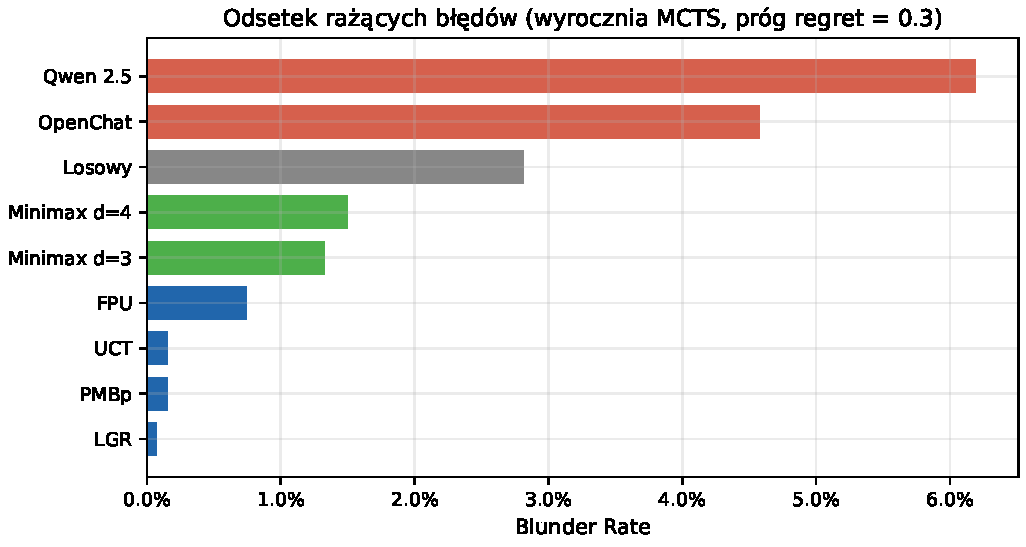
\includegraphics[width=0.88\textwidth]{figures/blunder_rate.pdf}
    \caption{Orientacyjny \textit{Blunder Rate} według agenta ($\tau = 0{,}3$, wyrocznia UCT $20\,000$ iteracji; patrz sekcja~\ref{sec:wyrocznia}).}
    \label{fig:blunder-rate}
\end{figure}

\begin{figure}[H]
    \centering
    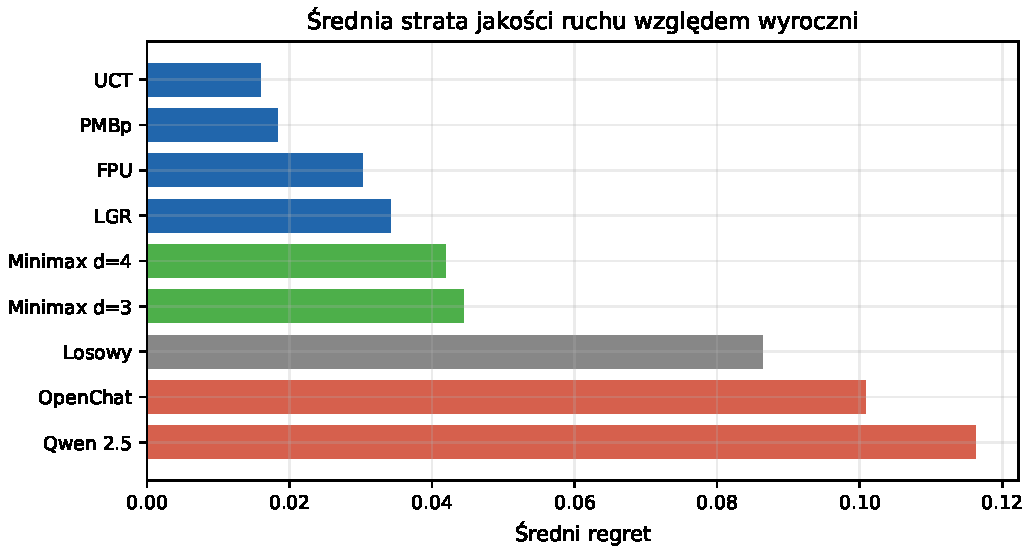
\includegraphics[width=0.88\textwidth]{figures/blunder_regret.pdf}
    \caption{Średni regret względem ruchu wskazanego przez wyrocznię (patrz sekcja~\ref{sec:wyrocznia}).}
    \label{fig:blunder-regret}
\end{figure}

Średni regret (rysunek~\ref{fig:blunder-regret}) jest najwyższy u LLM i gracza losowego, niższy u wariantów MCTS. Rysunek~\ref{fig:skill-vs-blunders} zestawia \textit{Win Rate} z orientacyjnym \textit{Blunder Rate} dla każdego agenta turniejowego; FPU ma 56{,}3\% wygranych przy wyższym odsetku blunderów wg wyroczni niż pozostałe warianty MCTS.

\begin{figure}[H]
    \centering
    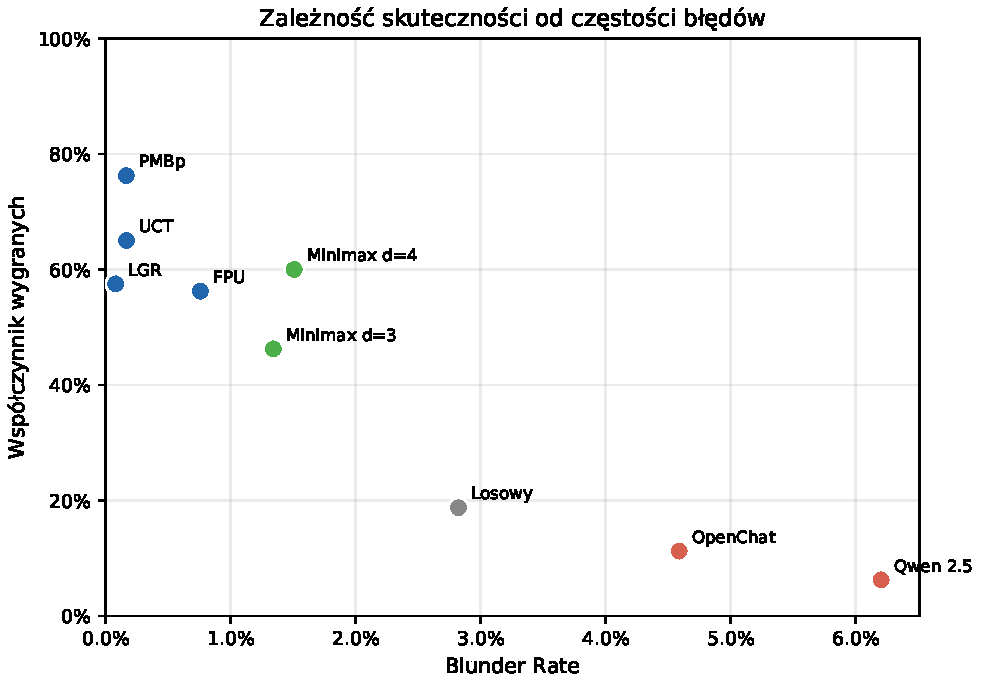
\includegraphics[width=0.82\textwidth]{figures/skill_vs_blunders.pdf}
    \caption{Zależność \textit{Win Rate} od orientacyjnego \textit{Blunder Rate} (każdy punkt to jeden agent turniejowy).}
    \label{fig:skill-vs-blunders}
\end{figure}



\subsection{Testy z udziałem człowieka i modeli językowych}
\label{sec:wyniki-czlowiek}

\subsubsection{Testy człowiek--komputer}

Pięciu uczestników rozegrało łącznie 70 partii przeciwko siedmiu agentom (po dwie gry na parę, z naprzemiennym kolorem). Tabela~\ref{tab:humans-vs-agents} zestawia współczynnik wygranych człowieka i agenta; rysunek~\ref{fig:humans-vs-agents} przedstawia te same dane graficznie.

\begin{table}[H]
    \centering
    \caption{Wyniki testów człowiek--komputer (10 partii na agenta, łącznie 70 gier).}
    \label{tab:humans-vs-agents}
    \small
    \begin{tabular}{lrrrr}
        \toprule
        \textbf{Agent} & \textbf{Wygrane człowieka} & \textbf{Wygrane agenta} & \textbf{Remisy} & \textbf{Win rate człowieka} \\
        \midrule
        Losowy & 10 & 0 & 0 & 100\% \\
        Minimax $d{=}3$ & 8 & 2 & 0 & 80\% \\
        Minimax $d{=}4$ & 3 & 3 & 4 & 30\% \\
        LGR & 3 & 5 & 2 & 30\% \\
        FPU & 2 & 5 & 3 & 20\% \\
        UCT & 1 & 7 & 2 & 10\% \\
        PMBp & 1 & 9 & 0 & 10\% \\
        \midrule
        \textbf{Łącznie} & 28 & 31 & 11 & 40{,}0\% \\
        \textbf{MCTS (razem)} & 7 & 26 & 7 & 17{,}5\% \\
        \bottomrule
    \end{tabular}
\end{table}

\begin{figure}[H]
    \centering
    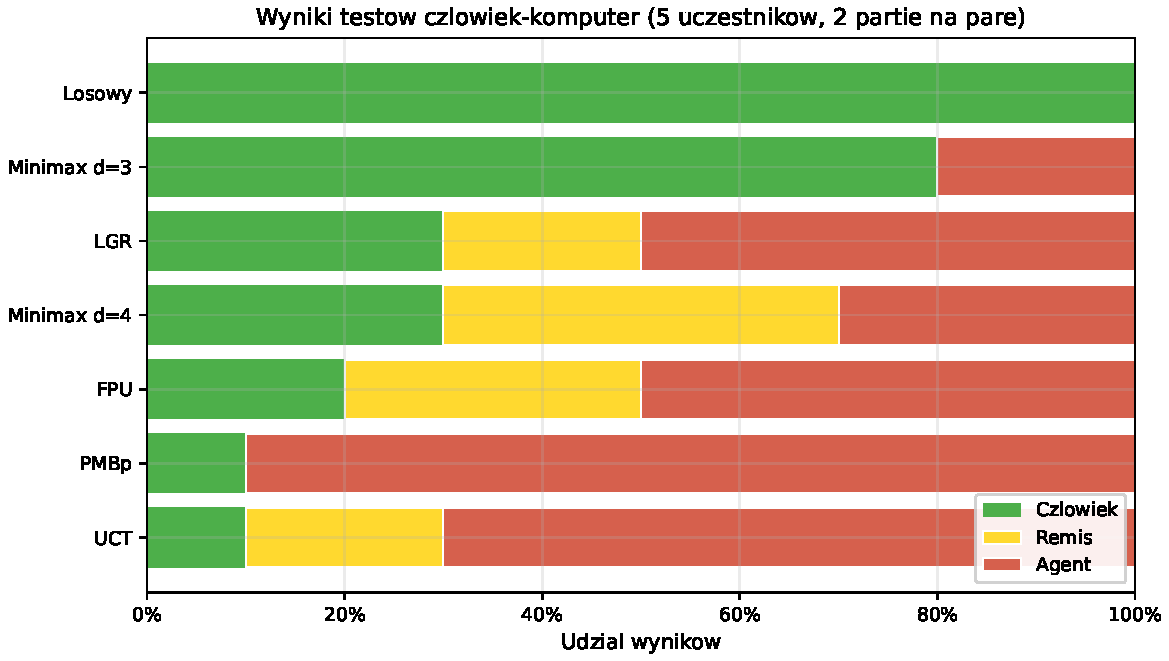
\includegraphics[width=0.92\textwidth]{figures/humans_vs_agents.pdf}
    \caption{Porównanie skuteczności człowieka i agenta w testach jeden na jeden (5 uczestników $\times$ 2 partie na parę; procent wygranych liczony wśród partii zakończonych zwycięstwem, bez remisów w mianowniku).}
    \label{fig:humans-vs-agents}
\end{figure}

Łączny \textit{Win Rate} człowieka jako czerwony wyniósł 31{,}4\% ($11/35$), jako żółty --- 48{,}6\% ($17/35$). Przeciwko wariantom MCTS uczestnicy wygrali 7 partii, przegrali 26 i zremisowali 7; przeciwko graczowi losowemu --- 10/10; przeciwko minimaxowi $d{=}3$ --- 8/10; przeciwko minimaxowi $d{=}4$ --- 3 wygrane, 3 porażki i 4 remisy.

\subsubsection{Porównanie między modelami językowymi}

W turnieju automatycznym modele \texttt{qwen2.5:7b} i \texttt{openchat:7b} osiągnęły odpowiednio 6{,}3\% i 11{,}3\% \textit{Win Rate} (po 80 partiach każdy). Gracz losowy miał 18{,}8\%. Średnia długość partii LLM wynosiła 13{,}3--18{,}2 ruchów. W bezpośrednich parach z agentami turniejowymi modele przegrywały większość gier; \texttt{openchat:7b} wygrał 3 z 10 partii z graczem losowym.

\begin{figure}[H]
    \centering
    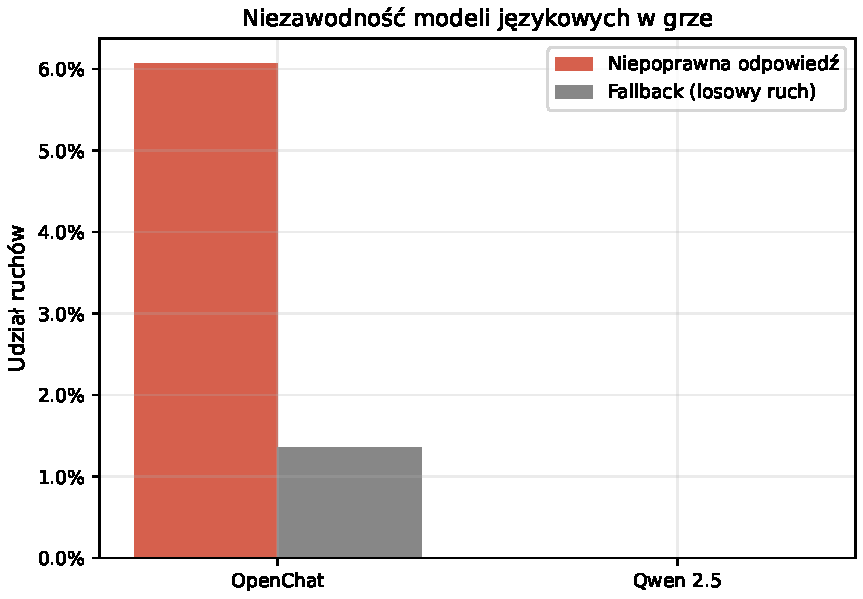
\includegraphics[width=0.78\textwidth]{figures/llm_reliability.pdf}
    \caption{Niezawodność odpowiedzi modeli językowych: odsetek niepoprawnych odpowiedzi API oraz ruchów losowych po błędzie (fallback).}
    \label{fig:llm-reliability}
\end{figure}

Metryki niezawodności interfejsu (rysunek~\ref{fig:llm-reliability}): OpenChat zwrócił niepoprawną odpowiedź w 6\% zapytań; Qwen 2.5 nie zanotował błędów parsowania i przegrał 75 z 80 partii w turnieju.

\subsection{Obserwacje dodatkowe}

\begin{itemize}
    \item \textbf{Remisy.} W parach MCTS--MCTS \textit{Draw Rate} w pojedynczych seriach sięgał 40--50\% (np.\ UCT--PMBp 5 remisów na 10 gier, UCT--FPU 4 na 10).

    \item \textbf{Czas decyzji.} FPU: ok.\ 1{,}51\,s/ruch; UCT i PMBp: ok.\ 1{,}26--1{,}28\,s; minimax $d{=}3$: 0{,}13\,s; minimax $d{=}4$: 0{,}63\,s (tabela~\ref{tab:tournament-summary}, rysunek~\ref{fig:decision-time}).

    \item \textbf{Tryb MCTS.} Agenci turniejowi nie utrzymywali drzewa między partiami; przed każdym ruchem wykonywano świeże przeszukiwanie z budżetem $1000$ iteracji.
\end{itemize}

\begin{figure}[H]
    \centering
    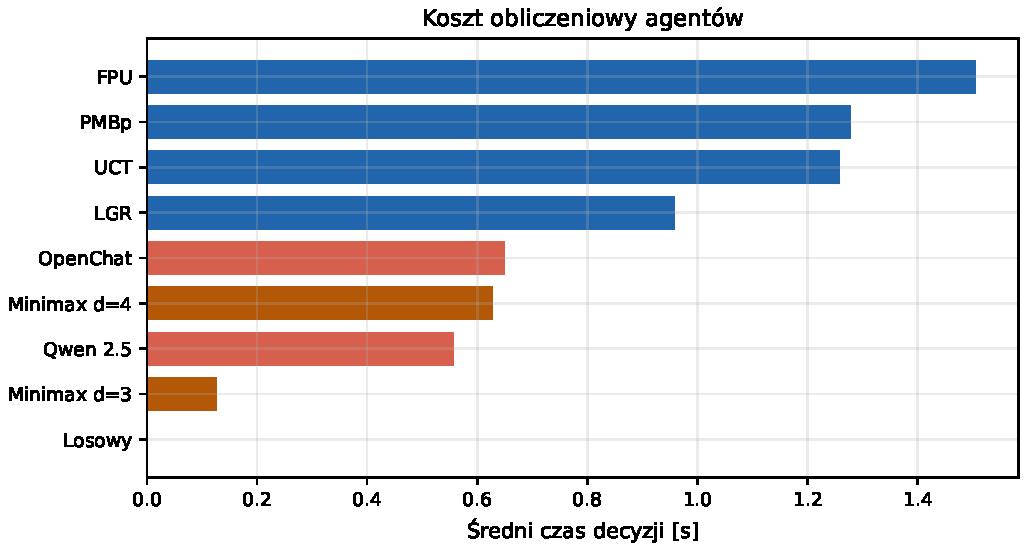
\includegraphics[width=0.85\textwidth]{figures/decision_time.pdf}
    \caption{Średni czas decyzji agentów w turnieju automatycznym.}
    \label{fig:decision-time}
\end{figure}

%----------------------------------------------------------------------------------------
%	5. WNIOSKI
%----------------------------------------------------------------------------------------
\section{Wnioski}

Poniżej podsumowujemy weryfikację hipotez z sekcji~\ref{sec:hipotezy-sformulowanie}, z wyraźnym rozróżnieniem między tym, co wynika z danych, a tym, co pozostaje otwarte ze względu na małą liczbę partii i ograniczenia metodologiczne.

\subsection{Weryfikacja hipotez}

\begin{enumerate}
    \item \textbf{Supremacja nad ludźmi i LLM --- częściowo potwierdzona.}
    \textit{Wobec LLM:} w turnieju każdy z czterech wariantów MCTS wygrywał z modelami językowymi w ponad 75\% partii bezpośrednich; OpenChat i Qwen 2.5 osiągnęły odpowiednio 11{,}3\% i 6{,}3\% \textit{Win Rate}. Próg 75\% jest spełniony dla MCTS \emph{vs} LLM w badanych warunkach (lokalne modele 7B, temperatura 1).

    \textit{Wobec człowieka:} próg 75\% zwycięstw MCTS \emph{nie} został spełniony --- w 40 partiach przeciwko czterem wariantom MCTS agenci wygrali 26 razy, uczestnicy 7 i zremisowano 7 (65\% wygranych MCTS w liczbie wszystkich partii). W 70 partiach łącznie ludzie wygrali 28 razy, przegrali 31 i zremisowali 11. Najwięcej wygranych człowieka przeciwko LGR (3/10) i FPU (2/10), najmniej przeciwko PMBp i UCT (po 1/10). Ci sami uczestnicy pokonali gracza losowego (10/10) i minimax $d{=}3$ (8/10); z minimaxem $d{=}4$ wynik to 3--3--4. Ogólna „supremacja AI nad człowiekiem” \emph{nie} została wykazana. Próba jest mała ($n{=}5$, 10 partii na agenta) i nie obejmuje graczy doświadczonych. 

    \textit{Uwaga:} hipoteza odnosiła się do MCTS w trybie online ($1000$ iteracji/ruch), a nie do agentów z długim treningiem self-play; wyniki nie należy utożsamiać z „wytrenowanym” silnikiem szachowym.

    \item \textbf{Przewaga UCT nad graczem heurystycznym --- częściowo potwierdzona.}
    W turnieju round-robin UCT (65{,}0\%) uzyskał wyższy \textit{Win Rate} niż minimax $d{=}4$ (60{,}0\%) i wyraźnie wyższy niż $d{=}3$ (46{,}3\%). W bezpośrednich parach: UCT--minimax $d{=}4$ to 5--2--3, UCT--minimax $d{=}3$ to 8--1--1. Różnica względem $d{=}4$ jest jednak umiarkowana (trzy remisy na dziesięć gier), a minimax $d{=}4$ wciąż plasuje się na trzecim miejscu w całym turnieju --- przed częścią wariantów MCTS. Hipotezę należy uznać za potwierdzoną względem słabszego minimaxa i prawdopodobną względem $d{=}4$, ale nie jako rozstrzygającą przewagę nad dobrze dobraną heurystyką.

    \item \textbf{Odporność PMBp na pułapki taktyczne --- nierozstrzygnięta (brak wiarygodnych danych).}
    Hipoteza wymaga porównania \textit{Blunder Rate} PMBp z innymi wariantami MCTS przy założeniu trafnej wyroczni. W eksperymencie wyrocznią był UCT z $20\,000$ iteracji na pozycję (sekcja~\ref{sec:wyrocznia}) --- rozwiązanie celowo uproszczone i prawdopodobnie \emph{stronnicze} wobec polityki UCT-a. Zaobserwowane wartości u silnych MCTS (0{,}08--0{,}76\%) odpowiadają jedynie kilku zdarzeniom na tysiąc ruchów; różnica między LGR (1 blunder) a PMBp i UCT (po 2) nie pozwala na żadne rzetelne wnioskowanie. FPU ma wyższy wskaźnik (9 blunderów), lecz bez niezależnej wyroczni nie wiadomo, czy jest to artefakt pomiaru.

    \textbf{Nie} uznajemy hipotezy za obaloną: brak dowodu na wyższą odporność PMBp nie jest dowodem na jej brak --- po prostu \textbf{nie zebrano danych} o jakości wymaganej do weryfikacji. Rozstrzygnięcie wymagałoby m.in.\ silniejszej lub bardziej bezstronnej wyroczni (np.\ głębszy minimax, większy budżet MCTS, analiza ludzka), większej liczby pozycji oraz ewentualnie niższego progu $\tau$ lub innych metryk jakości ruchu.

    \item \textbf{Zbalansowanie rozgrywki --- niejednoznaczna / słabo potwierdzona.}
    Wysoki \textit{Draw Rate} u silnych MCTS (do ok.\ 20\%, w parach MCTS--MCTS nawet 40--50\%) wskazuje na zacięty, defensywny charakter wariantu. Jednak kryterium z hipotezy --- \textit{Win Rate} gracza rozpoczynającego w przedziale 45--55\% --- nie jest spełnione u najlepszych agentów (PMBp: 72{,}5\% jako czerwony; UCT: 67{,}5\%). W testach ludzkich \textit{Win Rate} jako czerwony wyniósł 31{,}4\% ($11/35$), jako żółty --- 48{,}6\% ($17/35$). Plansza $6 \times 8$ łagodzi przewagę pierwszego ruchu względem klasycznego $6 \times 7$ w sposób jakościowy, lecz nie można twierdzić o pełnym zbalansowaniu w sensie liczbowym przyjętym w hipotezie.

    \item \textbf{Skuteczność modyfikacji UCT --- potwierdzona.}
    PMBp osiągnął 76{,}3\% \textit{Win Rate}, wyższy niż bazowy UCT (65{,}0\%), i wygrał bezpośrednie pojedynki z UCT (4--1--5), FPU (7--1--2) oraz LGR (7--1--2). FPU (56{,}3\%) i LGR (57{,}5\%) \emph{nie} przewyższyły UCT w rankingu ogólnym. Warunek hipotezy („co najmniej jedna modyfikacja”) jest spełniony przez PMBp; pozostałe modyfikacje w badanej konfiguracji nie poprawiły wyniku względem UCT.
\end{enumerate}

\subsection{Podsumowanie}

Zaimplementowano pełny pipeline do gry w wariant \textit{Connect4} typu suicide ($6 \times 8$, ruchy \texttt{drop}/\texttt{push}) z agentami MCTS (UCT, FPU, LGR, PMBp), minimaxem, graczem losowym i LLM, oraz wstępną metryką \textit{Blunder Rate} opartą o przybliżoną wyrocznię UCT. Eksperyment końcowy (360 partii turniejowych, ocena ok.\ 9400 ruchów, 70 gier człowiek--komputer) pozwala sformułować następujące wnioski ostrożne:

\begin{itemize}
    \item W badanym wariancie \textbf{PMBp z $p = 2{,}5$} okazał się najskuteczniejszym wariantem MCTS przy budżecie $1000$ iteracji/ruch, wyprzedzając bazowy UCT zarówno w rankingu round-robin, jak i w bezpośrednich parach.
    \item \textbf{MCTS w trybie online} wyraźnie przewyższa lokalne modele LLM w turnieju; w testach z człowiekiem wygrywa w większości partii przeciwko MCTS (26/40), lecz uczestnicy zdobyli też 7 zwycięstw i 7 remisów.
    \item \textbf{\textit{Blunder Rate}} w obecnej postaci (wyrocznia UCT, $\tau = 0{,}3$) z grubsza odróżnia słabych graczy od MCTS, lecz \textbf{nie pozwala} zweryfikować hipotezy o taktycznej przewadze PMBp --- metryka wymaga dalszego dopracowania, zanim stanie się narzędziem rozstrzygającym.
    \item \textbf{FPU} w tej konfiguracji ($\mathrm{FPU} = 1{,}0$) nie poprawił wyniku względem UCT w turnieju; wyższy \textit{Blunder Rate} wg wyroczni UCT-a nie jest wystarczającym dowodem gorszej gry taktycznej.
\end{itemize}

\textbf{Ograniczenia.} Po 10 partiach na parę wyniki turniejowe mają ograniczoną moc statystyczną; remisy i pojedyncze wyniki par mogłyby się zmienić przy dłuższym turnieju. Wyrocznia do \textit{Blunder Rate} jest świadomie przybliżona (UCT, skończony budżet, możliwa stronniczość) i nie zastępuje silniejszego silnika referencyjnego --- metryka nie rozstrzyga jakości ruchów między silnymi wariantami MCTS (sekcja~\ref{sec:wyrocznia}). Testy ludzkie ($n = 5$) przeprowadzono bez kontroli poziomu umiejętności uczestników. Modele LLM (7B, lokalnie) nie uogólniają się na populacje graczy ani na modele językowe. MCTS w turnieju nie był trenowany self-playem przed rozgrywką.

\textbf{Kierunki dalszych prac} obejmowałyby zwiększenie liczby partii i liczby ziaren losowości, trening trwałego drzewa przed turniejem, głębszy minimax lub uczenie funkcji oceny, powtórzenie testów ludzkich i z LLM na większej próbie i silniejszych modelach, oraz --- w kontekście hipotezy~3 --- zbudowanie \textbf{silniejszej i bardziej bezstronnej wyroczni} do \textit{Blunder Rate} (większy budżet, niezależna od ocenianego wariantu MCTS, ewentualnie weryfikacja na podzbiorze pozycji przez człowieka).

%----------------------------------------------------------------------------------------
%	Deklaracja użycia narzędzi sztucznej inteligencji
%----------------------------------------------------------------------------------------

\section{Deklaracja użycia narzędzi sztucznej inteligencji}
W ramach projektu modele językowe wykorzystano jako narzędzia pomocnicze podczas:
\begin{itemize}
    \item implementacji GUI oraz integracji gry z modelami językowymi,
    \item przygotowania skryptów przeprowadzających eksperymenty,
    \item opracowania wykresów i tabel z wynikami,
    \item przygotowania i formatowania roboczej bibliografii.
\end{itemize}

%----------------------------------------------------------------------------------------
%	BIBLIOGRAFIA
%----------------------------------------------------------------------------------------
\newpage
\bibliographystyle{plain}
\bibliography{bibliography}

\end{document}
